\chapter{The Client Perspective: Navigating Automation with Your Clients}


\section{Introduction}

As IT consultants, our success hinges not just on our technical expertise, but on our ability to guide clients through the transformative journey of automation. In this chapter, we'll explore how to effectively communicate the value of automation, address common concerns, and build long-lasting relationships with clients throughout their automation journey.


\section{Prospecting: Identifying Automation Opportunities}

When prospecting for new clients, it's crucial to approach potential automation projects with a keen eye for opportunity and value. Here's how to set the stage for successful automation discussions:

\subsection{Researching Potential Clients}

Before making initial contact, do your homework:

\begin{itemize}
    \item Use tools like Crunchbase or PitchBook to research the client's industry, funding, and growth trajectory
    \item Leverage LinkedIn Sales Navigator to identify key decision-makers and their professional backgrounds
    \item Use tools like Owler or SimilarWeb to gather competitive intelligence and industry trends
\end{itemize}

\subsection{Preparing Your Pitch}

Craft a compelling narrative around automation:

\begin{itemize}
    \item Use tools like Canva or Visme to create visually appealing case studies
    \item Develop an ROI calculator using Excel or Google Sheets, considering factors like time saved, error reduction, and productivity gains
    \item Create a "day in the life" video using tools like Loom or Vidyard to show how automation can transform their operations
\end{itemize}

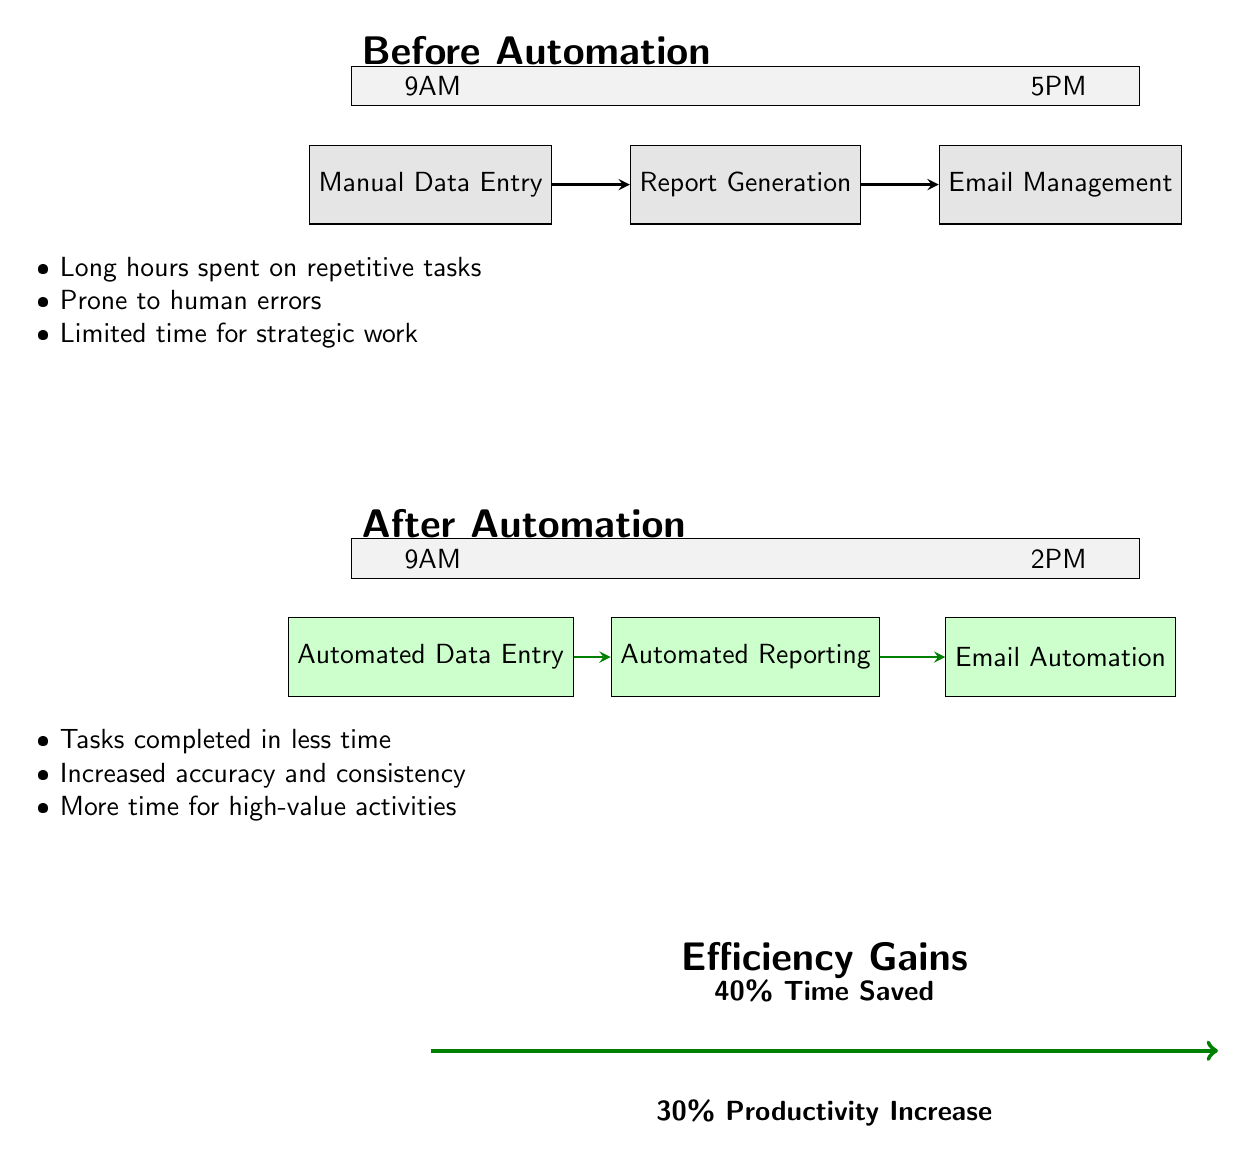
\begin{tikzpicture}[font=\sffamily]
        % Define styles
    \tikzset{
        task/.style={rectangle, minimum width=2cm, minimum height=1cm, draw, fill=gray!20},
        arrow/.style={->, >=stealth, thick},
        timebar/.style={rectangle, minimum width=10cm, minimum height=0.5cm, draw, fill=gray!10},
    }

    % Before Automation
    \node[anchor=north west] at (-6,4) {\Large\textbf{Before Automation}};
    \draw[timebar] (-6,3) rectangle (4,3.5) node[midway] {9AM \hspace{7cm} 5PM};

    \node[task] (manual1) at (-5,2) {Manual Data Entry};
    \node[task] (report1) at (-1,2) {Report Generation};
    \node[task] (email1) at (3,2) {Email Management};

    \draw[arrow] (manual1) -- (report1);
    \draw[arrow] (report1) -- (email1);

    \node[text width=10cm, align=left] at (-5,0.5) {
        \textbullet~Long hours spent on repetitive tasks\\
        \textbullet~Prone to human errors\\
        \textbullet~Limited time for strategic work
    };

    % After Automation
    \node[anchor=north west] at (-6,-2) {\Large\textbf{After Automation}};
    \draw[timebar] (-6,-3) rectangle (4,-2.5) node[midway] {9AM \hspace{7cm} 2PM};

    \node[task, fill=green!20] (auto1) at (-5,-4) {Automated Data Entry};
    \node[task, fill=green!20] (auto2) at (-1,-4) {Automated Reporting};
    \node[task, fill=green!20] (auto3) at (3,-4) {Email Automation};

    \draw[arrow, color=green!50!black] (auto1) -- (auto2);
    \draw[arrow, color=green!50!black] (auto2) -- (auto3);

    \node[text width=10cm, align=left] at (-5,-5.5) {
        \textbullet~Tasks completed in less time\\
        \textbullet~Increased accuracy and consistency\\
        \textbullet~More time for high-value activities
    };

    % Efficiency Gains
    \node[anchor=north] at (0,-7.5) {\Large\textbf{Efficiency Gains}};
    \draw[->, ultra thick, color=green!50!black] (-5,-9) -- (5,-9);
    \node[above=0.5cm] at (0,-9) {\textbf{40\% Time Saved}};
    \node[below=0.5cm] at (0,-9) {\textbf{30\% Productivity Increase}};
\end{tikzpicture}

\subsection{Targeting the Right Decision Makers}

Identify and approach the individuals who can champion automation within the organization:

\begin{itemize}
    \item Use LinkedIn to map out the organizational structure and identify potential champions
    \item Leverage LinkedIn's content creation tools to share thought leadership pieces on automation
    \item Engage with potential clients by commenting on their posts or sharing relevant articles
\end{itemize}


\section{Initial Contact: Making the Case for Automation}

The first interaction with a potential client is crucial. Here's how to make a strong first impression and begin the automation conversation:

\subsection{Opening the Dialogue}

Start the conversation by focusing on the client's needs, not your solutions:

\begin{itemize}
    \item Ask open-ended questions about their current challenges and goals
    \item Listen actively and take notes to demonstrate genuine interest
    \item Look for opportunities to naturally introduce the topic of automation
\end{itemize}

\subsection{Addressing Initial Skepticism}

Be prepared to encounter and address initial doubts:

\begin{itemize}
    \item "We're too small for automation" - Explain how automation can help small businesses compete with larger competitors
    \item "Automation is too expensive" - Demonstrate ROI and discuss flexible pricing models
    \item "We'll lose the personal touch" - Show how automation can free up time for more meaningful client interactions
\end{itemize}

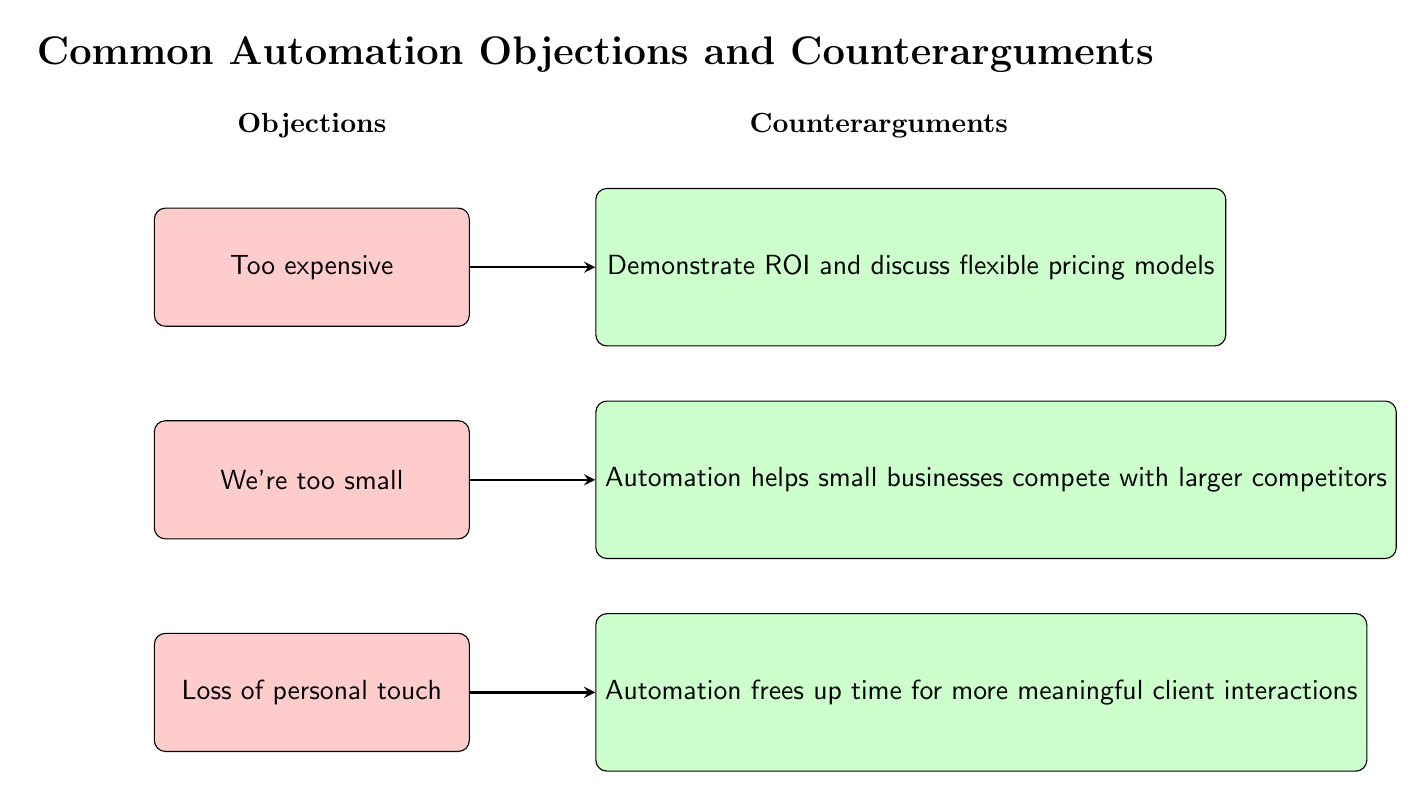
\begin{tikzpicture}[font=\sffamily, scale=0.9]
        % Define styles
    \tikzset{
        objection/.style={rectangle, rounded corners, minimum width=4cm, minimum height=1.5cm, draw, fill=red!20},
        counter/.style={rectangle, rounded corners, minimum width=8cm, minimum height=2cm, draw, fill=green!20},
        arrow/.style={->, >=stealth, thick},
    }

    % Title
    \node[font=\Large\bfseries] at (0,5) {Common Automation Objections and Counterarguments};

    % Labels
    \node[font=\bfseries] at (-4,4) {Objections};
    \node[font=\bfseries] at (4,4) {Counterarguments};

    % Objections and Counterarguments
    \node[objection] (obj1) at (-4,2) {Too expensive};
    \node[counter, anchor=west] (count1) at (0,2) {Demonstrate ROI and discuss flexible pricing models};

    \node[objection] (obj2) at (-4,-1) {We're too small};
    \node[counter, anchor=west] (count2) at (0,-1) {Automation helps small businesses compete with larger competitors};

    \node[objection] (obj3) at (-4,-4) {Loss of personal touch};
    \node[counter, anchor=west] (count3) at (0,-4) {Automation frees up time for more meaningful client interactions};

    % Arrows
    \draw[arrow] (obj1.east) -- (count1.west);
    \draw[arrow] (obj2.east) -- (count2.west);
    \draw[arrow] (obj3.east) -- (count3.west);
\end{tikzpicture}

\subsection{Demonstrating Value}

Use concrete examples and data to illustrate the potential of automation:

\begin{itemize}
    \item Share anonymized case studies from similar clients or industries
    \item Use visual aids to illustrate complex processes and how automation simplifies them
    \item If possible, offer a small-scale demonstration or proof of concept
\end{itemize}

% TODO @screenshot: A sample ROI calculator showing potential time and cost savings from an automation project


\section{Proposal: Crafting a Compelling Automation Strategy}

Once you've piqued the client's interest, it's time to develop a formal proposal. Here's how to create a proposal that addresses the client's needs and concerns:

\subsection{Tailoring the Solution}

Customize your automation proposal to the client's specific situation:

\begin{itemize}
    \item Use a CRM like HubSpot or Pipedrive to track client interactions and preferences
    \item Leverage proposal software like PandaDoc or Proposify to create professional, interactive proposals
    \item Use mind mapping tools like MindMeister or XMind to visualize and plan complex automation strategies
\end{itemize}

\subsection{Addressing Common Objections}

Proactively address potential concerns in your proposal:

\begin{itemize}
    \item Job displacement: Emphasize how automation frees up staff for more valuable work
    \item Data security: Detail the security measures in place, especially with self-hosted solutions
    \item Implementation complexity: Outline a clear, step-by-step implementation plan
    \item Disruption to work: Propose a gradual rollout to minimize disruption
\end{itemize}

\subsection{Highlighting Adaptability}

Emphasize the long-term adaptability of your proposed solution:

\begin{itemize}
    \item Explain how no-code solutions allow for quick adjustments as needs change
    \item Discuss how the proposed automation strategy prepares them for future technological shifts
    \item Outline a long-term partnership for ongoing optimization and scaling
\end{itemize}

\begin{tikzpicture}[node distance=2cm, auto, font=\sffamily]
        % Define styles
    \tikzset{
        block/.style={rectangle, draw, fill=blue!20,
        text width=5em, text centered, rounded corners, minimum height=3em},
        line/.style={draw, -latex'},
        cloud/.style={draw, ellipse, fill=red!20, minimum height=2em}
    }

    % Place nodes
    \node [block] (start) {Initial Process};
    \node [block, right of=start, xshift=3cm] (nocode) {No-Code Automation};
    \node [block, below of=nocode, yshift=-1cm] (change1) {Business Need Change};
    \node [block, right of=nocode, xshift=3cm] (adapt) {Quick Adaptation};
    \node [block, below of=adapt, yshift=-1cm] (change2) {New Technology};

    % Draw edges
    \path [line] (start) -- (nocode);
    \path [line] (nocode) -- (adapt);
    \path [line] (change1) -- (nocode);
    \path [line] (change2) -- (adapt);
    \path [line, dashed] (adapt) to [bend left=30] (nocode);

    % Add labels
    \node [above of=nocode, yshift=-1cm] {Easily Modifiable};
    \node [above of=adapt, yshift=-1cm] {Rapid Updates};

    % Add a cloud to represent flexibility
    \node [cloud, above of=start, yshift=1cm] {Flexible \& Scalable};
    \draw [-latex, dashed] (cloud) -- (nocode);
\end{tikzpicture}


\section{Implementation: Bringing Automation to Life}

Once the proposal is accepted, it's time to put your plan into action. Here's how to ensure a smooth implementation process:

\subsection{Setting Clear Expectations}

Start the implementation phase on the right foot:

\begin{itemize}
    \item Use project management tools like Asana or Trello to outline clear milestones and deadlines
    \item Set up regular check-ins to keep the client informed of progress
    \item Establish clear communication channels for questions and feedback
\end{itemize}

\subsection{Managing the Transition}

Guide the client through the change process:

\begin{itemize}
    \item Develop a change management plan to address potential resistance
    \item Provide comprehensive training on new automated systems
    \item Celebrate early wins to build momentum and enthusiasm
\end{itemize}

\subsection{Demonstrating Progress}

Keep the client engaged and confident throughout the implementation:

\begin{itemize}
    \item Use data visualization tools like Tableau or Power BI to create compelling progress reports
    \item Implement time-tracking tools to quantify time savings from automation
    \item Regularly showcase completed automations and their impact
\end{itemize}

% TODO @screenshot: A sample project dashboard showing implementation progress, completed milestones, and realized benefits


\section{Ongoing Support and Optimization}

The journey doesn't end with implementation. Here's how to provide ongoing support and continue delivering value:

\subsection{Proactive Maintenance}

Stay ahead of potential issues:

\begin{itemize}
    \item Set up monitoring and alerting systems using n8n
    \item Conduct regular health checks on automated systems
    \item Proactively suggest optimizations based on usage data
\end{itemize}

\subsection{Continuous Improvement}

Keep refining and expanding the automation:

\begin{itemize}
    \item Regularly reassess the client's business needs and goals
    \item Propose new automations or expansions of existing ones
    \item Stay informed about new features or integrations that could benefit the client
\end{itemize}

\subsection{Building Long-Term Partnerships}

Transform your role from service provider to trusted advisor:

\begin{itemize}
    \item Offer strategic consulting on digital transformation
    \item Provide insights on industry trends and emerging technologies
    \item Host workshops or seminars to keep clients educated and engaged
\end{itemize}


\section{Case Study: Transforming a Skeptical Client into an Automation Advocate}

Let's examine how one IT consultant successfully navigated a challenging client relationship:

\begin{itemize}
    \item Initial skepticism: The client was hesitant about automation, fearing job losses and disruption
    \item Tailored approach: The consultant focused on automating tedious tasks first, demonstrating immediate value
    \item Gradual expansion: As trust grew, more complex automations were implemented
    \item Results: 40% increase in productivity, 25% cost savings, and the client became a vocal advocate for automation
\end{itemize}

\begin{tikzpicture}[font=\sffamily, scale=0.8]
    % Define styles
    \tikzset{
        milestone/.style={circle, draw, fill=blue!20, minimum size=1cm},
        event/.style={rectangle, rounded corners, draw, fill=green!20, minimum width=4cm, minimum height=1.5cm, text width=3.8cm, align=center},
        arrow/.style={->, >=stealth, thick},
    }

    % Draw timeline
    \draw[very thick] (-1,0) -- (12,0);
    \foreach \x in {0,3,...,12}
    \draw (\x,0.2) -- (\x,-0.2);

    % Milestones
    \node[milestone] (m1) at (0,0) {1};
    \node[milestone] (m2) at (3,0) {2};
    \node[milestone] (m3) at (6,0) {3};
    \node[milestone] (m4) at (9,0) {4};
    \node[milestone] (m5) at (12,0) {5};

    % Events
    \node[event, above=0.8cm of m1] (e1) {Initial Skepticism};
    \node[event, below=0.8cm of m2] (e2) {First Automation};
    \node[event, above=0.8cm of m3] (e3) {Expanded Adoption};
    \node[event, below=0.8cm of m4] (e4) {Measurable Results};
    \node[event, above=0.8cm of m5] (e5) {Automation Advocate};

    % Connect events to timeline
    \foreach \i in {1,2,3,4,5}
    \draw[arrow] (e\i) -- (m\i);

    % Add labels
    \node[below=0.3cm] at (m1) {Month 1};
    \node[below=0.3cm] at (m3) {Month 6};
    \node[below=0.3cm] at (m5) {Month 12};

    % Add details
    \node[text width=3.8cm, align=center, above=0.2cm] at (e1) {Fear of job losses and disruption};
    \node[text width=3.8cm, align=center, below=0.2cm] at (e2) {Automated tedious tasks};
    \node[text width=3.8cm, align=center, above=0.2cm] at (e3) {Implemented more complex automations};
    \node[text width=3.8cm, align=center, below=0.2cm] at (e4) {40\% productivity increase 25\% cost savings};
    \node[text width=3.8cm, align=center, above=0.2cm] at (e5) {Client promotes automation to peers};

    % Title
    \node[font=\Large\bfseries] at (6,5) {Client's Automation Journey};
\end{tikzpicture}


\section{Conclusion}

Successfully implementing automation for clients is about much more than just technical know-how. It's about building trust, demonstrating value, and fostering a long-term partnership focused on continuous improvement and adaptation.

By following the strategies outlined in this chapter, you'll be well-equipped to guide your clients through every stage of their automation journey, from initial skepticism to long-term success.

\textbf{Action Items}:
\begin{enumerate}
    \item Develop a "automation readiness" questionnaire to use during the prospecting phase
    \item Create a template for an automation proposal that addresses common objections
    \item Design a basic training program for a common automation scenario
    \item Set up a system for regular check-ins and optimization reviews with existing clients
\end{enumerate}

Remember, every client's journey with automation will be unique. Stay flexible, keep learning, and always focus on delivering real, measurable value. Your success as an IT consultant in the age of automation depends on your ability to be a trusted guide, helping your clients navigate the exciting possibilities of this ever-evolving landscape.

% TODO @qr: QR code linking to additional resources on client communication and relationship management in automation projects